\section{Vision meets Language in Geometric Agentic Reasoning}

% Slide 15: Geometry is where everything collides
\begin{frame}{Geometry is where everything collides}
  \begin{columns}[T]
    \column{0.48\textwidth}
    \begin{itemize}
      \item Vision + Language + Planning + Tool use
      \item Algebraic reasoning alone is not enough
      \item Spatial relationships require true understanding
      \item The hardest setting — where all earlier problems converge
    \end{itemize}

    \column{0.52\textwidth}
    \centering
    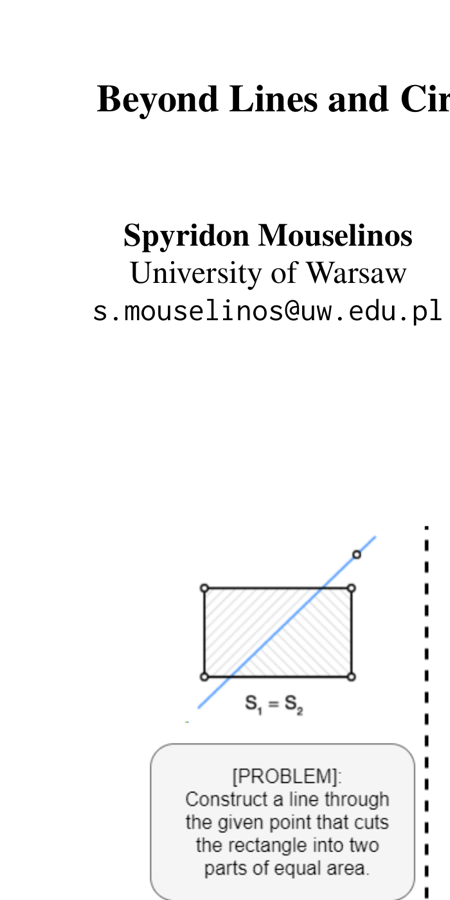
\includegraphics[height=0.7\textheight,keepaspectratio]{assets/euclidea-problem-screenshot}
    \vspace{-0.3em}
    {\tiny Source: Euclidea game screenshot}
  \end{columns}
  \note{Geometry is the culmination of the dissertation. It is not just another benchmark. It combines visual understanding, symbolic reasoning, sequential planning, and tool use in one open-ended task. Models that look strong in algebra or text often struggle here, because constructive geometry is a much stricter test of reasoning.}
\end{frame}

% Slide 17: Single-model prompting: not enough
\begin{frame}{Single-model prompting: not enough}
  \begin{itemize}
    \item Zero-shot hallucinated tools
    \item Static few-shot copied styles and steps
    \item Adaptive few-shot selected better prior problems
    \item Geometry made planning failures very visible
    \item \textbf{ChatGPT: 5.9 → 13.6 with best prompting}
  \end{itemize}
  \begin{center}
    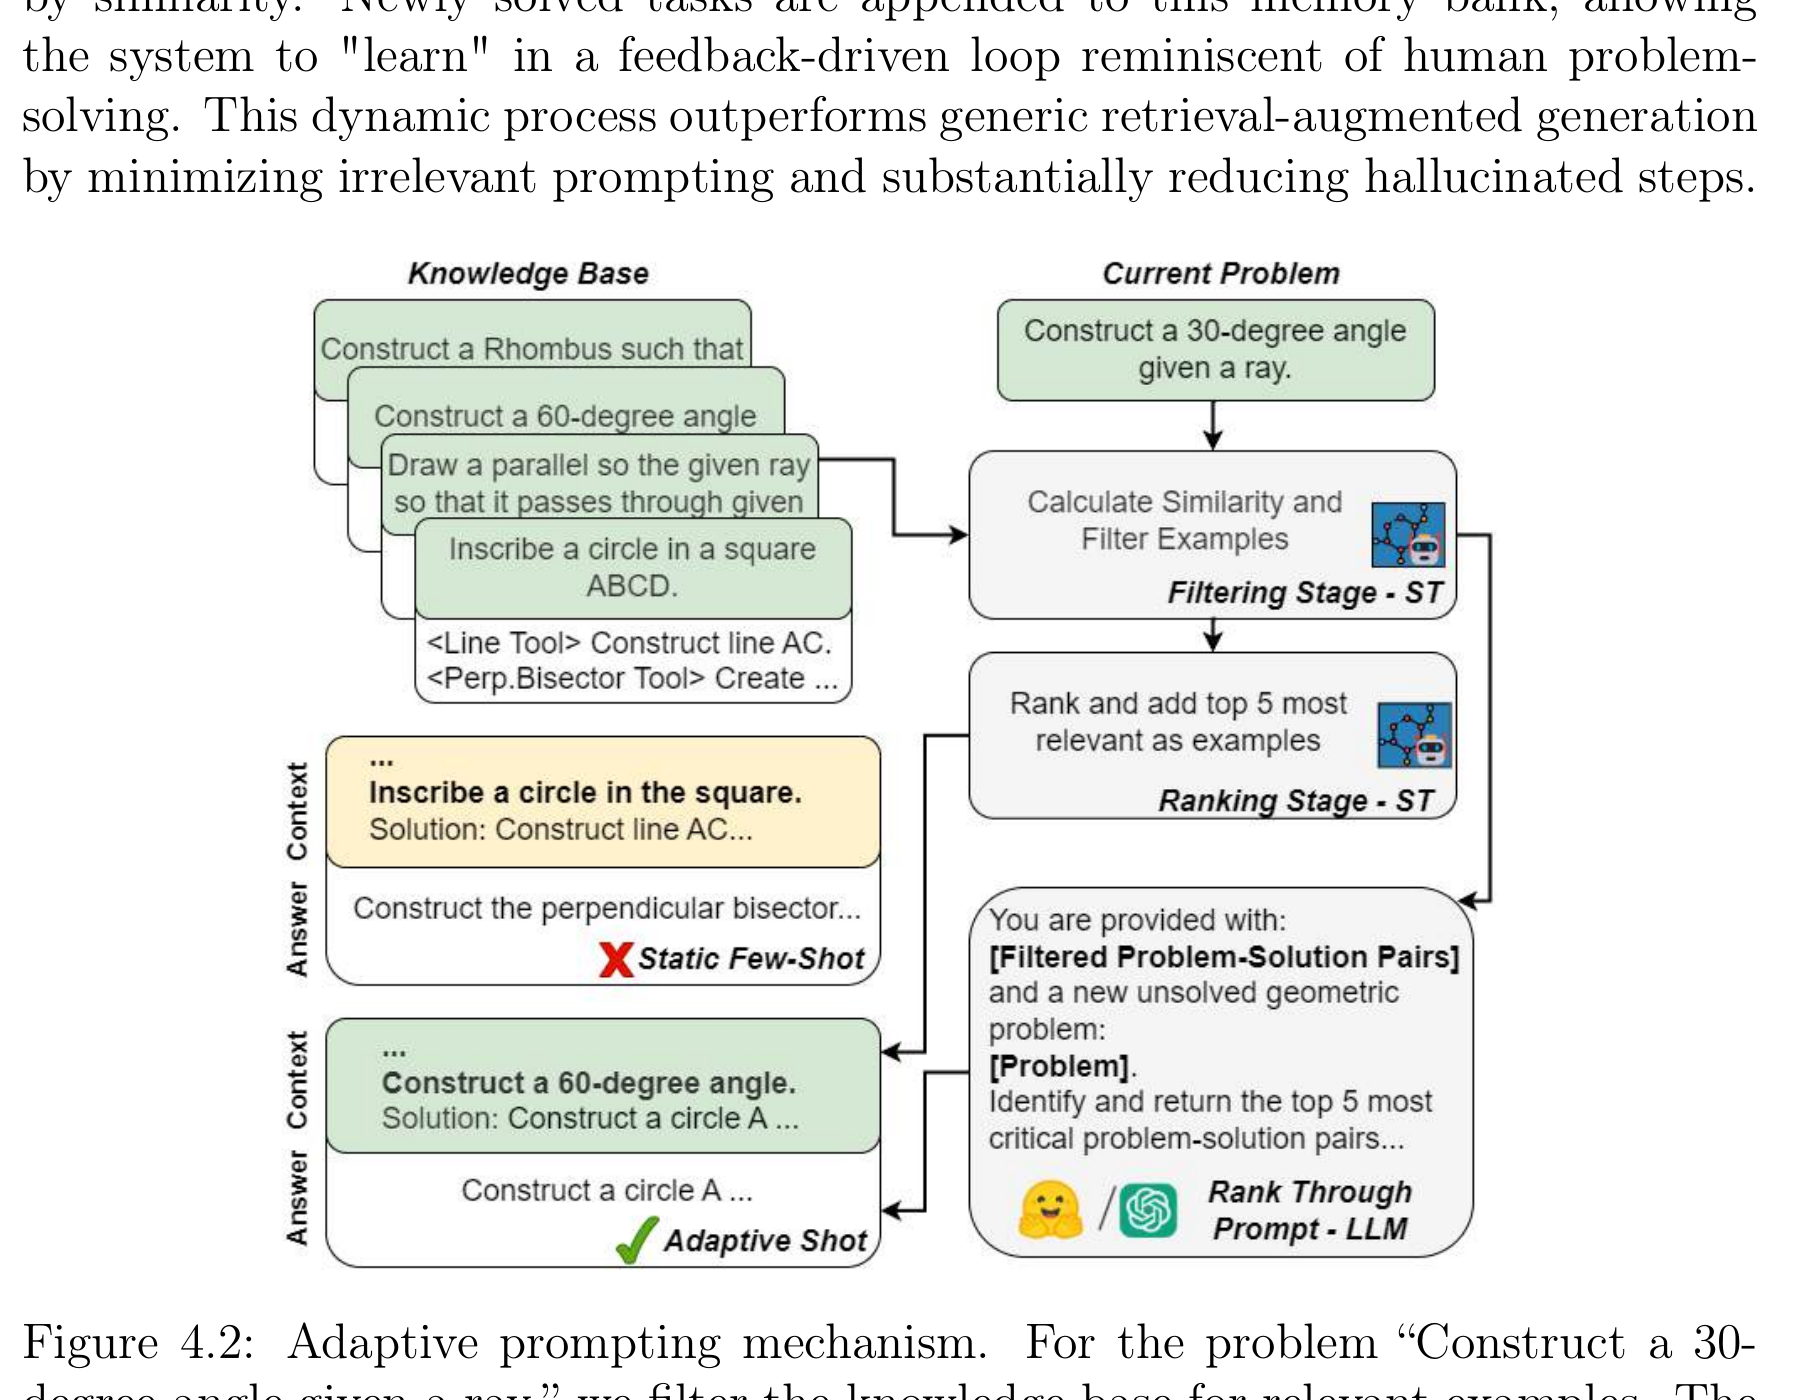
\includegraphics[width=0.7\textwidth,height=0.5\textheight,keepaspectratio]{assets/thesis-fig-4-2-baselines}
    \vspace{-0.3em}
    {\tiny Source: Thesis Fig. 4.2 (baseline prompting results)}
  \end{center}
  \note{I first studied what goes wrong before building the full system. Zero-shot prompting often hallucinated tool behavior. Static few-shot reduced that, but it introduced another problem: the model copied the style and even the reasoning path of the prompt examples. Adaptive few-shot helped by retrieving more relevant demonstrations. In the ablations, ChatGPT improves from 5.9 zero-shot to 13.6 with Adaptive-Shot Self on Alpha and Beta levels.}
\end{frame}

% Slide 18: From monologue to teamwork
\begin{frame}{From monologue to teamwork}
  \begin{itemize}
    \item Natural-language solver plans
    \item Geometry-tool solver executes
    \item Validators critique and refine
    \item Specialization separates reasoning from action
  \end{itemize}
  \begin{center}
    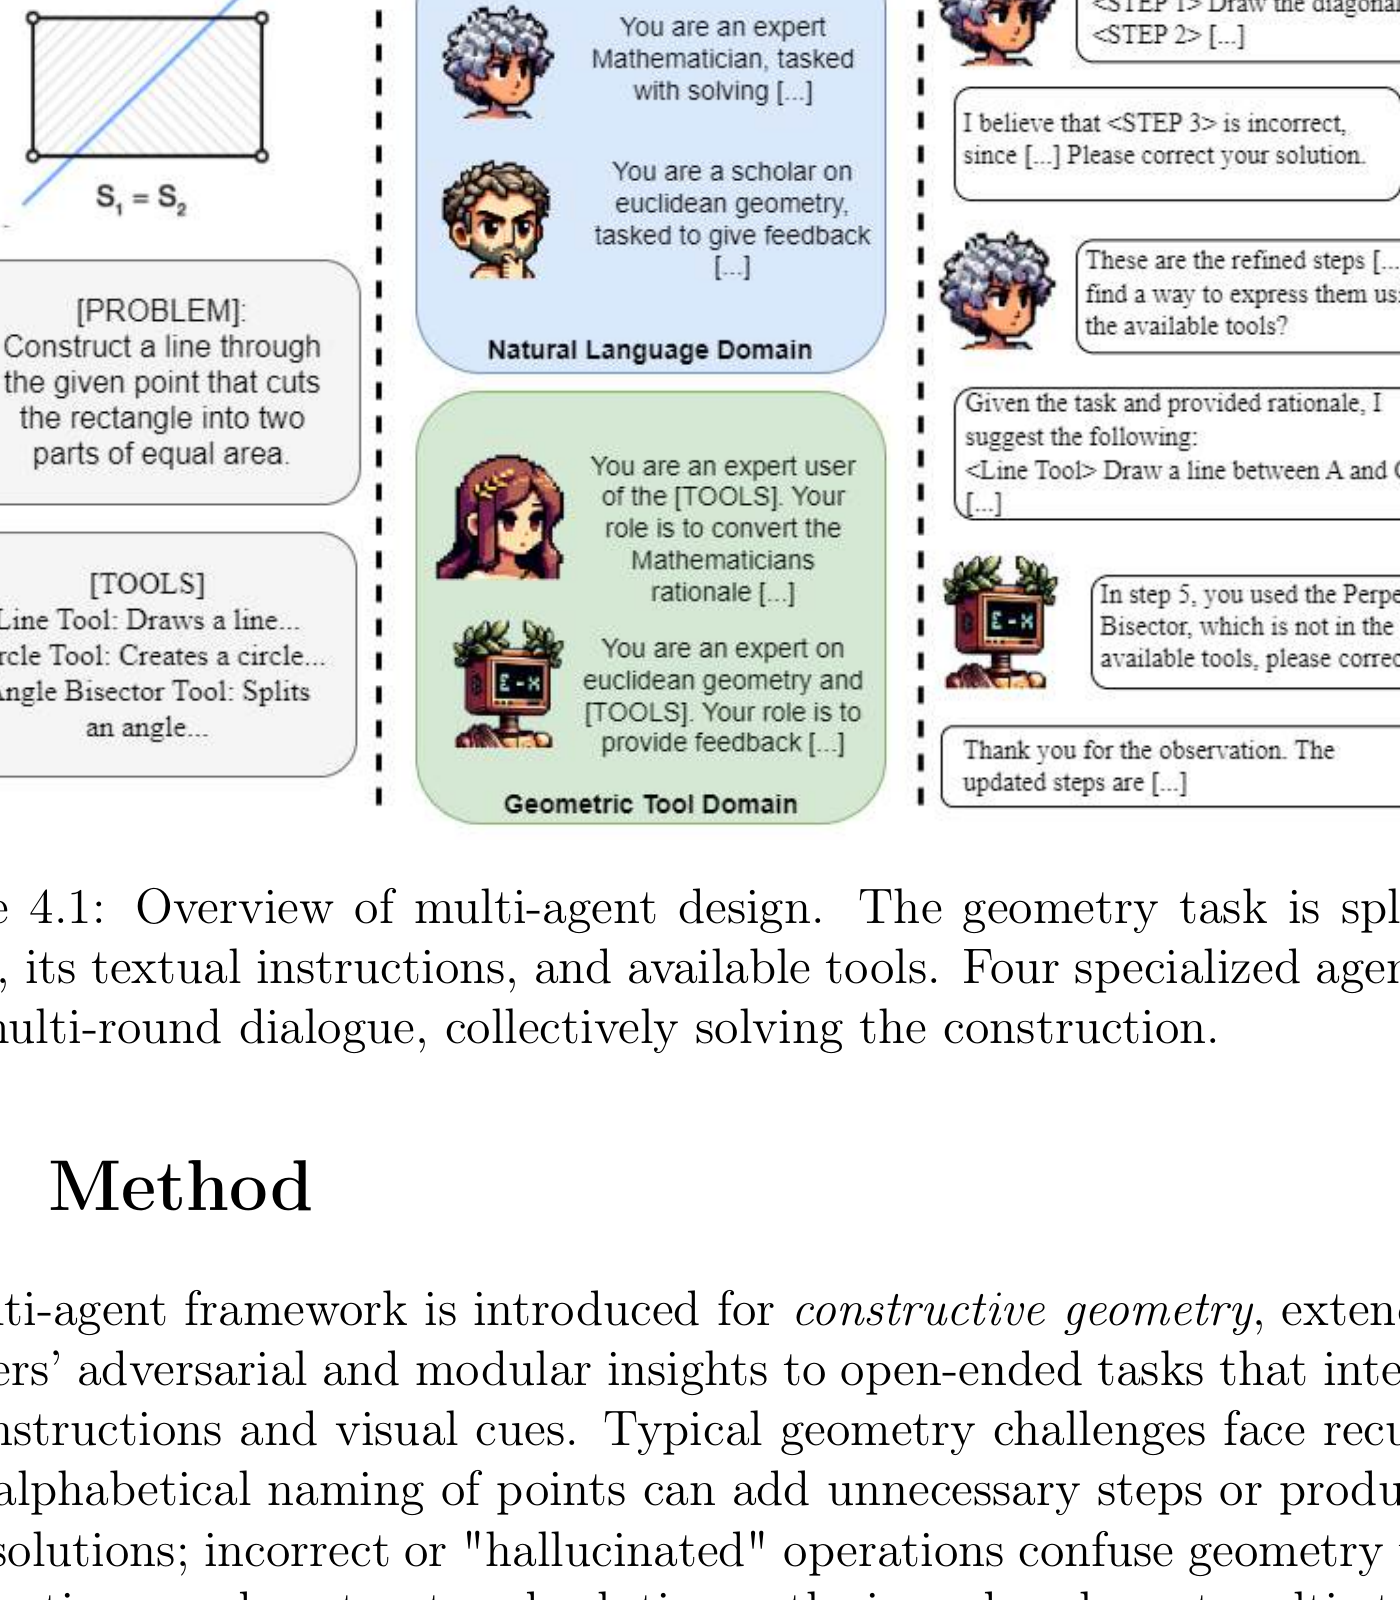
\includegraphics[height=0.7\textheight,keepaspectratio]{assets/thesis-fig-4-1-multi-agent-arch}
    \vspace{-0.3em}
    {\tiny Source: Thesis Fig. 4.1 (multi-agent architecture)}
  \end{center}
  \note{This is the conceptual heart of the geometry chapter. I stop treating the model as one monolithic reasoner and instead organize the reasoning process. One agent plans in natural language, another translates that plan into geometric tool steps, and validators criticize both levels. The key idea is that reasoning improves when we structure it — not only when we scale the model.}
\end{frame}

% Slide 19: Two more failure modes: grounding and naming
\begin{frame}{Two more failure modes: grounding and naming}
  \begin{columns}
    \column{0.5\textwidth}
    \begin{itemize}
      \item VRP converts the image into explicit spatial relations
      \item VLM perception alone was not enough
      \item Variable names can distort solution length and stopping
      \item Renaming the target to X reduces bias
    \end{itemize}

    \column{0.5\textwidth}
    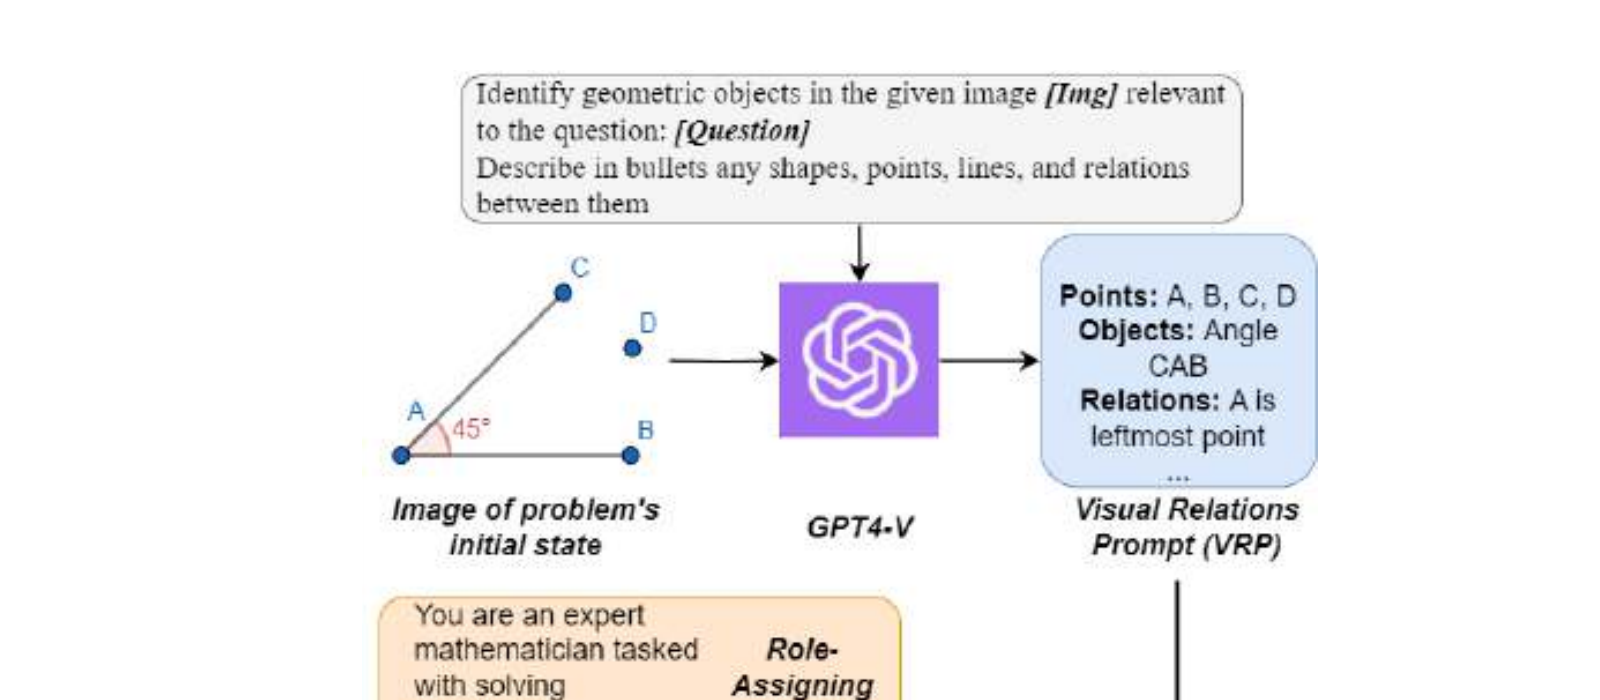
\includegraphics[width=\textwidth,height=0.35\textheight,keepaspectratio]{assets/thesis-fig-4-3-vrp-clean}
    \vspace{-0.2em}
    {\tiny Source: Thesis Fig. 4.3 (VRP)}

    \vspace{0.3em}

    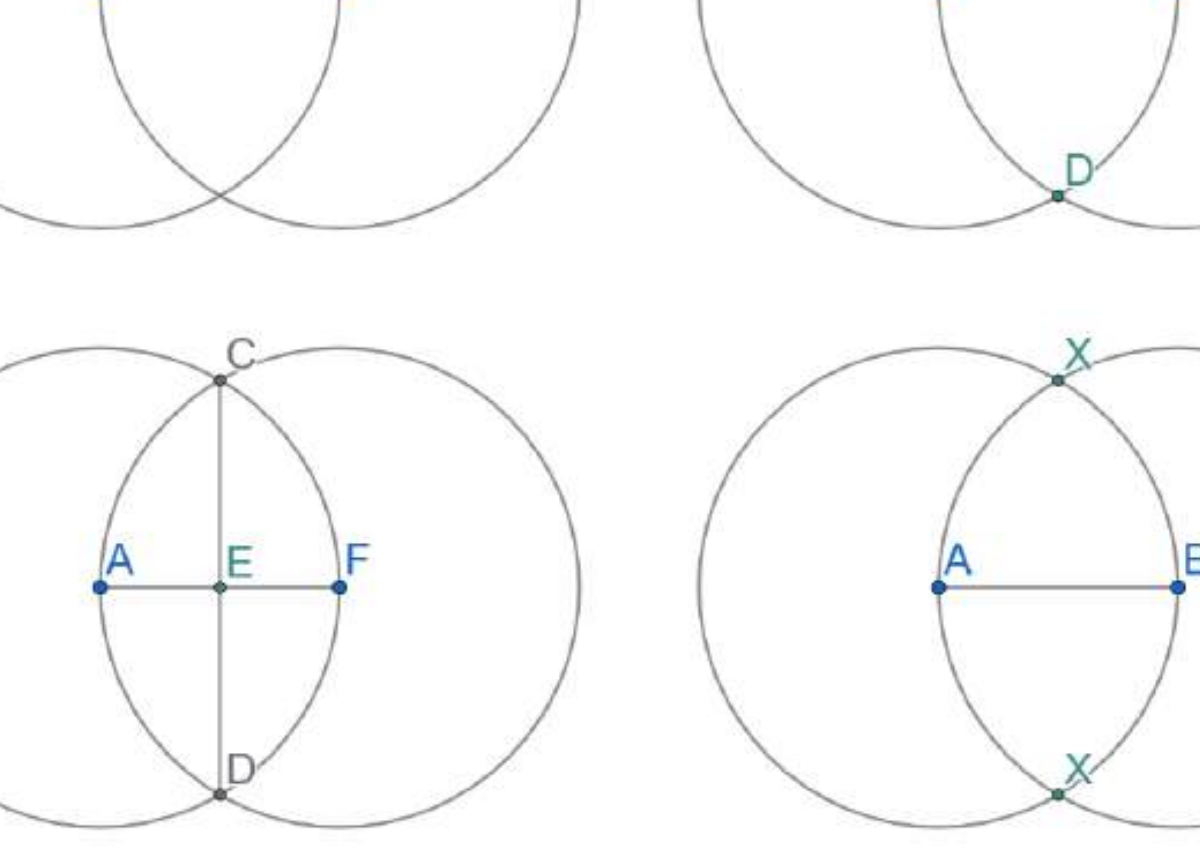
\includegraphics[width=\textwidth,height=0.35\textheight,keepaspectratio]{assets/thesis-fig-4-4-naming-bias-clean}
    \vspace{-0.2em}
    {\tiny Source: Thesis Fig. 4.4 (naming bias)}
  \end{columns}
  \note{I found two more very specific failure modes. First, even multimodal models could recognize scene elements but still fail to integrate them into a valid construction plan. The Visual Relations Prompt fixes that by turning the image into explicit relations in language. Second, alphabetical naming created a bias: target labels like C, D, or E could distort the reasoning path. Replacing the target with X often restored shorter, cleaner solutions.}
\end{frame}

% Slide 18: What the Geometry Chapter Taught Me
\begin{frame}{What the Geometry Chapter Taught Me}
  \begin{itemize}
    \item Multi-agent structure beats single prompting
    \item Role and domain specialization matter
    \item VRP and feedback loops help further
    \item The framework transfers beyond geometry
  \end{itemize}
  \begin{center}
    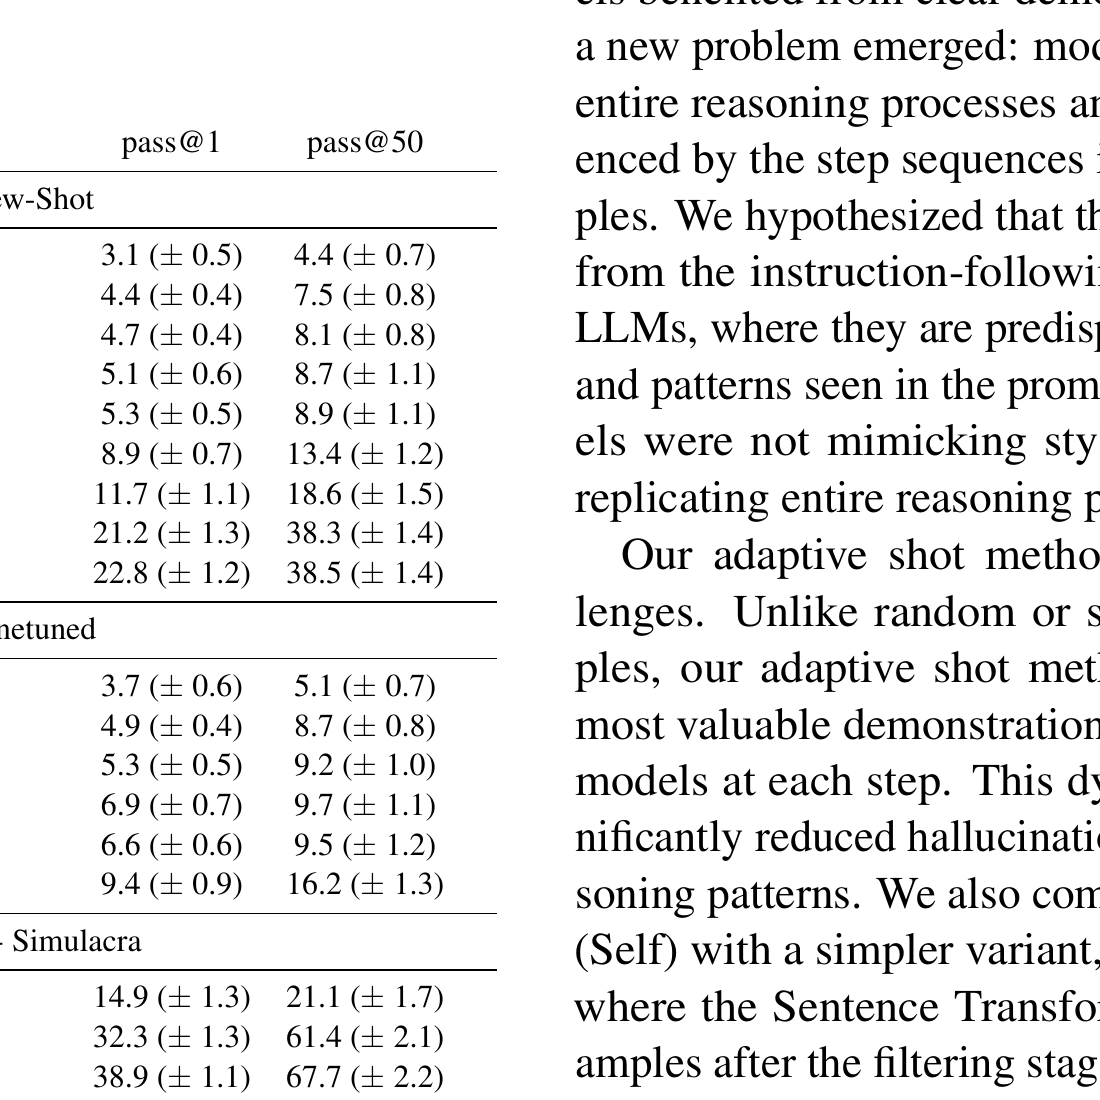
\includegraphics[width=0.7\textwidth,height=0.5\textheight,keepaspectratio]{assets/emnlp-table-1-cropped}
    \vspace{-0.3em}
    {\tiny Source: EMNLP 2024 Table 1 (Euclidea results and transfer)}
  \end{center}
  \note{This slide is the culmination of the thesis. The gains are large, and the ablations explain why: domain separation, validators, VRP, and naming neutralization all contribute. Importantly, the framework is not just a geometry trick. By swapping tools, it also transfers to GSM8K, SVAMP, and MATH-style reasoning tasks. The broader lesson is that structure and collaboration can extend the reasoning limits of general-purpose models. This serves as the explicit synthesis for the geometry chapter: structure matters as much as scale, and multi-agent specialization is a constructive answer to the limitations exposed in the earlier chapters. The claim that it 'transfers beyond geometry' is supported by the generalization results table showing performance on algebraic reasoning tasks.}
\end{frame}
